

\documentclass{article}
\usepackage{qilin}
\tikzstyle{process} = [rectangle, rounded corners, minimum width=1.5cm, minimum height=0.5cm,align=center, draw=black, fill=gray!30, auto]
\title{\vspace{-2cm}MAT357: Real Analysis \\ Problem Set 4}
\author{QiLin Xue}
\date{2022-2023}
\usepackage{mathrsfs}
\usetikzlibrary{arrows}
\usepackage{stmaryrd}
\usepackage{accents}
\newcommand{\ubar}[1]{\underaccent{\bar}{#1}}
\usepackage{pgfplots}
\numberwithin{equation}{section}

\begin{document}

\maketitle
I worked with Ahmad, Jonah, and Nathan on this problem set.
\begin{enumerate}
    \item \begin{enumerate}[label=(\alph*)]
        \item No discontinuities - \textbf{TRUE.} By Theorem 1 of the book.
        \item At most 10 discontinuities - \textbf{TRUE.} We will show that if $f$ has more than 10 discontinuities, then there exists an $N\in \mathbb{N}$ such that $n>N$ implies that $f_n$ has more than 10 discontinuities.
        
        Suppose that $f$ has a discontinuity at $x_0$. This means that there exists an $\epsilon > 0$, any for any $\delta > 0,$ we have $|x-a|<\delta$ implies that 
        \begin{equation}
            |f(x_0)-f(a)| > \epsilon.
        \end{equation}
        We now claim that there exists an $N\in \mathbb{N}$ such that $n>N$ implies that $f_n$ also has a discontinuity at $x_0.$ We prove this by contradiction. Suppose that $f_n$ is continuous at $x_0.$ Then for any $\epsilon > 0$ there exists $\delta' > 0$ such that $|x_0-a|<\delta \implies |f_n(x_0)-f_n(x_0)|< \frac{\epsilon}{10}.$ Note that if $\delta'$ works then so does 
        \begin{equation}
            \delta'' = \text{min}\{\delta',\delta\},
        \end{equation}
        where $\delta$ is picked from the $\epsilon$ before. Due to convergence (we only require point-wise convergence here), we know that there exists $N\in \mathbb{N}$ such that $n>N$ implies that 
        \begin{align}
            |f_n(x_0)- f(x_0)| < \frac{\epsilon}{10},|f_n(a)- f(a)| < \frac{\epsilon}{10}.
        \end{align}
        We can bring everything together using the triangle inequality. Given the $\epsilon > 0$ from before (when we showed that $f$ has a discontinuity at $x_0$), we have $|x-a|<\delta''$ implies that 
        \begin{equation}
            |f(x)-f(a)| \le |f(x) - f_n(x)| + |f_n(x) - f_n(a)| + |f_n(a) - f(a)| < \frac{\epsilon}{10} + \frac{\epsilon}{10} + \frac{\epsilon}{10} = \frac{3\epsilon}{10} < \epsilon.
        \end{equation}
        But we showed before that $ |f(x)-f(a)|,$ giving us a contradiction. Because every discontinuity in the limit function corresponds to the same discontinuity in the sequence, we know this is true.

        We can choose an $N_i$ for each discontinuity $x_1,\dots,x_k$ in $f,$ and by the above for $N> \text{max}\{N_i\}$, we have that $f_n$ has at least $k$ discontinuities. Therefore, if $f$ were to have more than 10 discontinuities, then we can find $f_n$ with more than 10 discontinuities.
        \item At least 10 discontinuities - \textbf{FALSE.} Let $[a,b]=[0,10]$ and consider the sequence 
        \begin{equation}
            f_n(x) = \frac{1}{n}\lfloor x\rfloor.
        \end{equation} 
        This has 10 discontinuities, at $x=1,2,\ldots,10.$ However, they converge to $f(x) = 0,$ which has no discontinuities. We just need to show that it is uniform convergence. This is true since for any $\epsilon > 0,$ we can choose $N = \frac{100}{\epsilon}$ such that for $n>N,$ we have:
        \begin{align}
            \text{sup}|f_n(x) - f(x)| &= \text{max}f_n(x) \\ 
            &< \text{max}f_N(x) \\ 
            &= \frac{10}{N} \\ 
            &< \frac{\epsilon}{10} < \epsilon.
        \end{align}
        % \item Finitely many discontinuities: \textbf{FALSE.}
        % Let $[a,b]=[0,1].$ First define $\tilde{C}_n(x)$ to be 
        % \begin{equation}
        %     \tilde{C}_n(x) = \begin{cases}
        %         0 & x \in C_n(x) \\ 
        %         1 & x \notin C_n(x)
        %     \end{cases}
        % \end{equation}
        % where $C_n(x)$ is the middle-thirds Cantor set defined on $[0,1].$ Then define $f_n(x)$ to be 
        % \begin{equation}
        %     f_n(x) = \sum_{i=1}^{n} \frac{\tilde{C}_i(x)}{2^i}.
        % \end{equation}
        % First, we will show that $f_n(x)$ converges to 
        % \begin{equation}
        %     f(x) = \sum_{i=1}^{\infty}\frac{\tilde{C}_i(x)}{2^i}.
        % \end{equation}
        % Note that for every $x,$ we know that $f(x)$ exists since if $\tilde{C}_k(x) = 1$ then $\tilde{C}_i(x) = 1$ for all $i \ge k.$ This is because the middle-thirds Cantor set is constructed by removing intervals, and so if a point is already not contained in it, removing intervals will preserve this. There are two cases:
        % \begin{itemize}
        %     \item If $\tilde{C}_i(x) =0 $ for all $i\in \mathbb{N}$ then it's obvious that $f(x)=0$
        %     \item Let $k \in \mathbb{N}$ be the first index such that $\tilde{C}_i(x)=1,$ then:
        %     \begin{equation}
        %         f(x) = \sum_{i=k}^{\infty}\frac{1}{2^i} < 1 
        %     \end{equation}
        %     and converges as it is an infinite geometric sum.
        % \end{itemize}
        % For each $f_n(x),$ we have a finite number of discontinuities, however it converges to $f(x).$ We can show that $f(x)$ has a countably number of discontinuities. Specifically, $f_n(x)$ has $2(2^{n}-1)$ discontinuities.
        % \begin{proof}
             


        %     Prove my induction. If $n=1$ then we clearly have $2$ discontinuities. Now suppose this is true for $n=k.$ Then for $n=k+1,$ we are looking a
        % \end{proof}
        \item Finitely many discontinuities: \textbf{False}. Let $[a,b]=[0,1].$ Consider the function 
        \begin{equation}
            f_n(x) = \begin{cases}
                x & x \in \left\{\frac{1}{1},\frac{1}{2},\ldots,\frac{1}{n}\right\} \\
                0 & \text{else}
            \end{cases}
        \end{equation}
        and define 
        \begin{equation}
            f(x) = \begin{cases}
                x & x \in \{1,1/2,1/3,\dots\} \\ 
                0 & \text{else}.
            \end{cases}
        \end{equation}
        Clearly, $f_n(x)$ has $n$ discontinuities and the limit function $f(x)$ has a countable (infinite) number of discontinuities. We now need to show that $f_n(x)$ uniformly converges to $f(x).$ We do so by computing the sup-norm,
        \begin{equation}
            \text{sup}|f(x)-f_n(x)| = \frac{1}{n},
        \end{equation}
        which approaches $0$ as $n \to \infty.$
        \item Countably many jump discontinuities: \textbf{True.} In fact, we will prove that there cannot be uncountably many jump discontinuities. To do so, note that jump discontinuities are isolated points. This is because $x_0$ is a jump discontinuity if and only if 
        \begin{equation}
            \lim_{x\to x_0^-}f(x) \neq \lim_{x\to x_0^+}f(x),
        \end{equation}
        but they both exist. But for the one-sided limits to exist, you need to be able to construct an interval $(x_0-\delta,x_0)$ and $(x_0,x_0+\delta)$ where the function is continuous, i.e. the point $x_0$ is isolated from any other discontinuity.

        Now consider the set of all jump discontinuities $\{x_\alpha\}$, which form isolated points. In other words, the distance between any two discontinuities $x,y$ is nonzero (actually, we need a stronger statement: that for any discontinuity we can have an open interval around it such that it only contains this. This is true because the continuities are jump). To prove that this set is countable, consider $\mathbb{Q}.$ For each $q\in \mathbb{Q}$ consider $x = \text{min}\{x\in \{x_\alpha\}| x>q\}.$ This minimum exists since all the points are isolated. Now consider the open set around $q,$
        \begin{equation}
            (q-\epsilon_1, x + \epsilon_2),
        \end{equation}
        which contains $x$ but doesn't contain any other discontinuity. This can be done because the discontinuities are isolated, so there's some finite distance between any two of them. This creates an injection from $\{x_\alpha\} \to $ so $\{x_\alpha\}$ must be countable. Therefore, there cannot be uncountable many jump discontinuities and the number of jump discontinuities is countable.
        \item No jump discontinuities: \textbf{False.} Consider the function 
        \begin{equation}
            f_n(x) = \begin{cases}
                1 & x \le 0 \\ 
                \frac{1}{n}\sin(1/x) & x > 0.
            \end{cases}
        \end{equation}
        For every $f_n(x)$ there is a discontinuity at $x=0,$ but it is not a jump discontinuity because $\lim_{x\to 0^+} \frac{1}{n}\sin(1/x)$ does not exist. However, the function converges to 
        \begin{equation}
            f(x) = \begin{cases}
                1 & x \le 0 \\ 
                0 & x > 0,
            \end{cases}
        \end{equation}
        which has a jump discontinuity at $x=0.$ Finally, we need to verify that this convergence is uniform. Note that the function doesn't change for $x\le 0 ,$ so 
        \begin{align}
            \text{sup}\{f_n(x)-f(x)\} = \text{sup}\{\frac{1}{n}\sin(1/x) - 0\} = \frac{1}{n},
        \end{align}
        which approaches $0$ as $n\to \infty.$
        \item No oscillating discontinuities: \textbf{True}. Suppose that $f_n(x)$ has no oscillating discontinuities. That means all discontinuities are jump discontinuities.
        
        We prove the contrapositive. Suppose the limit function $f(x)$ has an oscillating discontinuity at $x_0.$ There are two cases:
        \begin{itemize}
            \item Case 1: $x_0$ is a hole, i.e. it is removable. Specifically, $\lim_{x\to x_0^+}f(x) = \lim_{x\to x_0^-}f(x),$ but they are not equal to $f(x_0).$ We can apply the same reasoning as in (b) to show that if we have a removable discontinuity in $f(x)$ then for some $N\in \mathbb{N},$ $n>N$ implies that there is a jump discontinuity at $f_n(x_0).$ I didn't work out the details fully here.
            \item Case 2: $x_0$ is some other discontinuity: This means that either $\lim_{x\to x_0^+}f(x)$ or $\lim_{x\to x_0^-}$ is not defined, or both. WLOG, take $\lim_{x\to x_0^+}f(x)$ to be undefined. Then we claim that there exists $N\in \mathbb{N}$ such that $n>N$ implies that $\lim_{x\to x_0^+}f_n(x)$ is undefined. If it was defined, then uniform convergence requires that the points around this limit approach to $f(x)$ at a rate that can be bounded (i.e. ``slowly''). I didn't have time to work out the rest of the details here either, but I suspect it is similar to a $\delta-\epsilon$ proof as in part (b).
        \end{itemize}
    \end{enumerate}
    % \item To do this, we need the following lemma:
    % \begin{lemma}
    %     If $\{g_n(x)\}$ is equicontinuous and $\{h_n(x)\}$ is equicontinuous, then $\{g_n(x)+h_n(x)\}$ is equicontinuous, where $g_n,h_n:\mathbb{R}\to \mathbb{R}.$
    %     \begin{proof}
    %         TODO
    %     \end{proof}
    % \end{lemma}
    % \begin{lemma}
    %     If $\{g_n(x)\}$ is equicontinuous and $h:\mathbb{R}\to\mathbb{R}$ is continuous, then $\{f(g_n(x))\}$ is continuous, where $g_n,h_n:\mathbb{R}\to \mathbb{R}.$
    %     \begin{proof}
    %         TODO
    %     \end{proof}
    % \end{lemma}
    % Suppose that $\{f_n(x)\}$ was equicontinuous. Then by the above lemmas, we must have that 
    % \begin{equation}
    %     \left\{\sqrt{\sqrt{n+2}(\exp\left(f_n(x)- \cos(n+x)\right)-1)}=\sin(n^nx)\right\}
    % \end{equation}
    % is equicontinuous. If $\{g_n(x)\}$ is equicontinuous over $\mathbb{R},$ it should also be equicontinuous over some interval. Restrict $|n^n x|<1,$ and appl 
    % \item We will show that $f_n(x)$ is not equicontinuous by showing that at $x=0$ it is not equicontinuous. Then $f_n(x)=\cos(n)$ for all $n\in \mathbb{N}.$ Now let us pick $\epsilon = \frac{1}{2}.$ Then for any $\delta > 0$ there exists $n\in \mathbb{N}$
    \newpage
    \item We will prove that it is equicontinuous. We will use the following lemma:
    \begin{lemma}
        The sequence $g_n(x)=\frac{\sin^2(n^n x)}{\sqrt{n+2}}$ is equicontinuous.
        \begin{proof}
            Let $\epsilon > 0.$ Since $g_n(x)$ converges to $0$ as $n\to \infty,$ there exists $N\in \mathbb{N}$ such that for all $n>N,$ we have $g_n(x) < \epsilon.$ Namely, pick 
            \begin{equation}
                N = \left\lfloor \frac{1}{\epsilon^2}-2 \right\rfloor. 
            \end{equation}
            Then,
            \begin{align}
                |g_n(x_0) - g_n(a)| &> \left|\frac{1}{\sqrt{n+2}} - 0\right| \\ 
                &> \frac{1}{\sqrt{N+2}} \\ 
                &> \epsilon.
            \end{align}
            So for $n>N,$ we are done automatically for any $\delta.$ Now let us work with the $n \le N$ case. Because $g(x)$ is continuous, for any $n \le N,$ there exists a $\delta_n$ that ensures 
            \begin{equation}
                |s-t| <\delta_n \implies |g_n(s)-g_n(t)| < \epsilon.
            \end{equation}
            Therefore, define 
            \begin{equation}
                \delta = \text{min}\{\delta_i:i=1,\dots, N\}.
            \end{equation}
            Clearly, $g_n(x)$ converges with the same $\delta$ for all $n \le N.$ Therefore, we have shown that $g_n(x)$ is equicontinuous.
        \end{proof}
    \end{lemma}
    We can add $1$ to each element in the sequence $g_n(x)=\frac{\sin^2(n^n x)}{\sqrt{n+2}},$ and we will still get an equicontinuous sequence (i.e. shift by constant). We can now prove that 
    \begin{equation}
        \log(1+g_n(x))
    \end{equation}
    is equicontinuous in a similar way. For any $\epsilon > 0,$ we pick the same $N\in \mathbb{N}$ as in the lemma. For $n>N$ we know that 
    \begin{equation}
        0 < \log(1 + g_n(x)) < \log(1 + \epsilon) < \epsilon
    \end{equation}
    so by the same reasoning as before, $|\log(1+g_n(x_0)) < \log(1+g_n(a))| < \epsilon$ for any $\delta.$ Then for the $n\le N$ case, we use the same trick of finding the minimum $\delta_n$ and defining $\delta = \text{min}\{\delta_i:i=1,\dots, N\}.$
    \begin{lemma}
        If $f_n(x)$ is equicontinuous and $g_n(x)$ is equicontinuous, then $f_n(x)+g_n(x)$ is equicontinuous.
        \begin{proof}
            For any $\epsilon/2 > 0,$ there exists $\delta',\delta'' > 0$ such that 
            \begin{equation}
                |x-a| < \delta' \implies |f_n(x)-f_n(a)| < \epsilon/2
            \end{equation} 
            and 
            \begin{equation}
                |x-a| < \delta'' \implies |g_n(x)-g_n(a)| < \epsilon/2.
            \end{equation}
            Pick $\delta=\text{min}\{\delta',\delta''\}$ such that 
            \begin{align}
                |x-a| < \delta \implies |f_n(x)+g_n(x)-f_n(a)-g_n(a)| &< |f_n(x) - f_n(a)| + |g_n(x) - g_n(a)| \\
                &< \epsilon/2 + \epsilon/2 \\
                &= \epsilon.
            \end{align}
        \end{proof}
    \end{lemma}
    Also note that $\cos(n+x)$ is equicontinuous. A standard first-year calculus result will show that setting $\delta=\epsilon$ is sufficient. This does not depend on $\delta$ so $\cos(n+x)$ is equicontinuous. The sum of two equicontinuous sequences is equicontinuous, so we can conclude that 
    \begin{equation}
        \cos(n+x)+\log\left(1 + \frac{1}{\sqrt{n+2}}\sin^2(n^nx)\right)
    \end{equation}
    is equicontinuous.
    \item \begin{enumerate}
        \item For every $\epsilon > 0,$ we can pick $\delta = \left(\frac{\epsilon}{H}\right)^{1/\alpha}.$ Then the set $C^{\alpha}(H)$ of continuous functions defined on $[a,b]$ with $\alpha$-Holder constant $\le H$ is equicontinuous because 
        \begin{align}
            |s-t| < \delta,n\in \mathbb{N} &\implies |s-t| < \left(\frac{\epsilon}{H}\right)^{1/\alpha} \\ 
            &\implies H|s-t|^\alpha < \epsilon.  
        \end{align}
        Because each function $f_i$ is $\alpha$-Holder continuous, we have
        \begin{equation}
            |s-t| < H_i|f_i(s)-f_i(t)|^\alpha < H|f_i(s)-f_i(t)|^\alpha,
        \end{equation}
        since the $H_i$ for each function is bounded above by $H.$ But we have shown that $H|s-t|^\alpha < \epsilon,$ so this $\delta$ implies that 
        \begin{equation}
            |s-t| < \delta \implies |f_i(s)-f_i(t)| < \epsilon.
        \end{equation} 
        \item The same proof applies.
        \item The same proof applies.
    \end{enumerate}
    \newpage
    \item \begin{enumerate}[label=(\alph*)]
        \item  Consider $g(x) = \text{sup}\{f(x):f\in \mathcal{E}\}.$ Because $\mathcal{E}$ is uniformly continuous, given some $\epsilon'=\epsilon/10,$ there exists a $\delta > 0$ such that $|x_0-a|<\delta \implies |f(x_0)-f(a)|<\epsilon'=\epsilon/10$ for all $f \in \mathcal{E}.$ Now we will prove that $g(x)$ is continuous.
    
        For any $\epsilon > 0,$ pick the $\delta>0$ that corresponds to $\epsilon'=\epsilon/10$ for the functions in $\mathcal{E},$ as per above. Then we can show that $g(x)$ is continuous at $x_0.$ Because $g(x)$ is the least upper bound, there exist functions $h(x),k(x)$ that are within $\epsilon/10$ at $x_0$ and $a$ respectively. 
    
        Because $h(x),k(x)$ are equicontinuous, then $|x_0-a|<\delta$ implies that $|h(x_0) - k(a)|<\epsilon/10$ which implies that $|h(x_0)-h(a)|<\epsilon/10.$ Similarly, the same thing goes for $k(x)$ so that $|h(x_0)-h(a)|<\epsilon/10.$ We get the following diagram:
        \begin{center}
            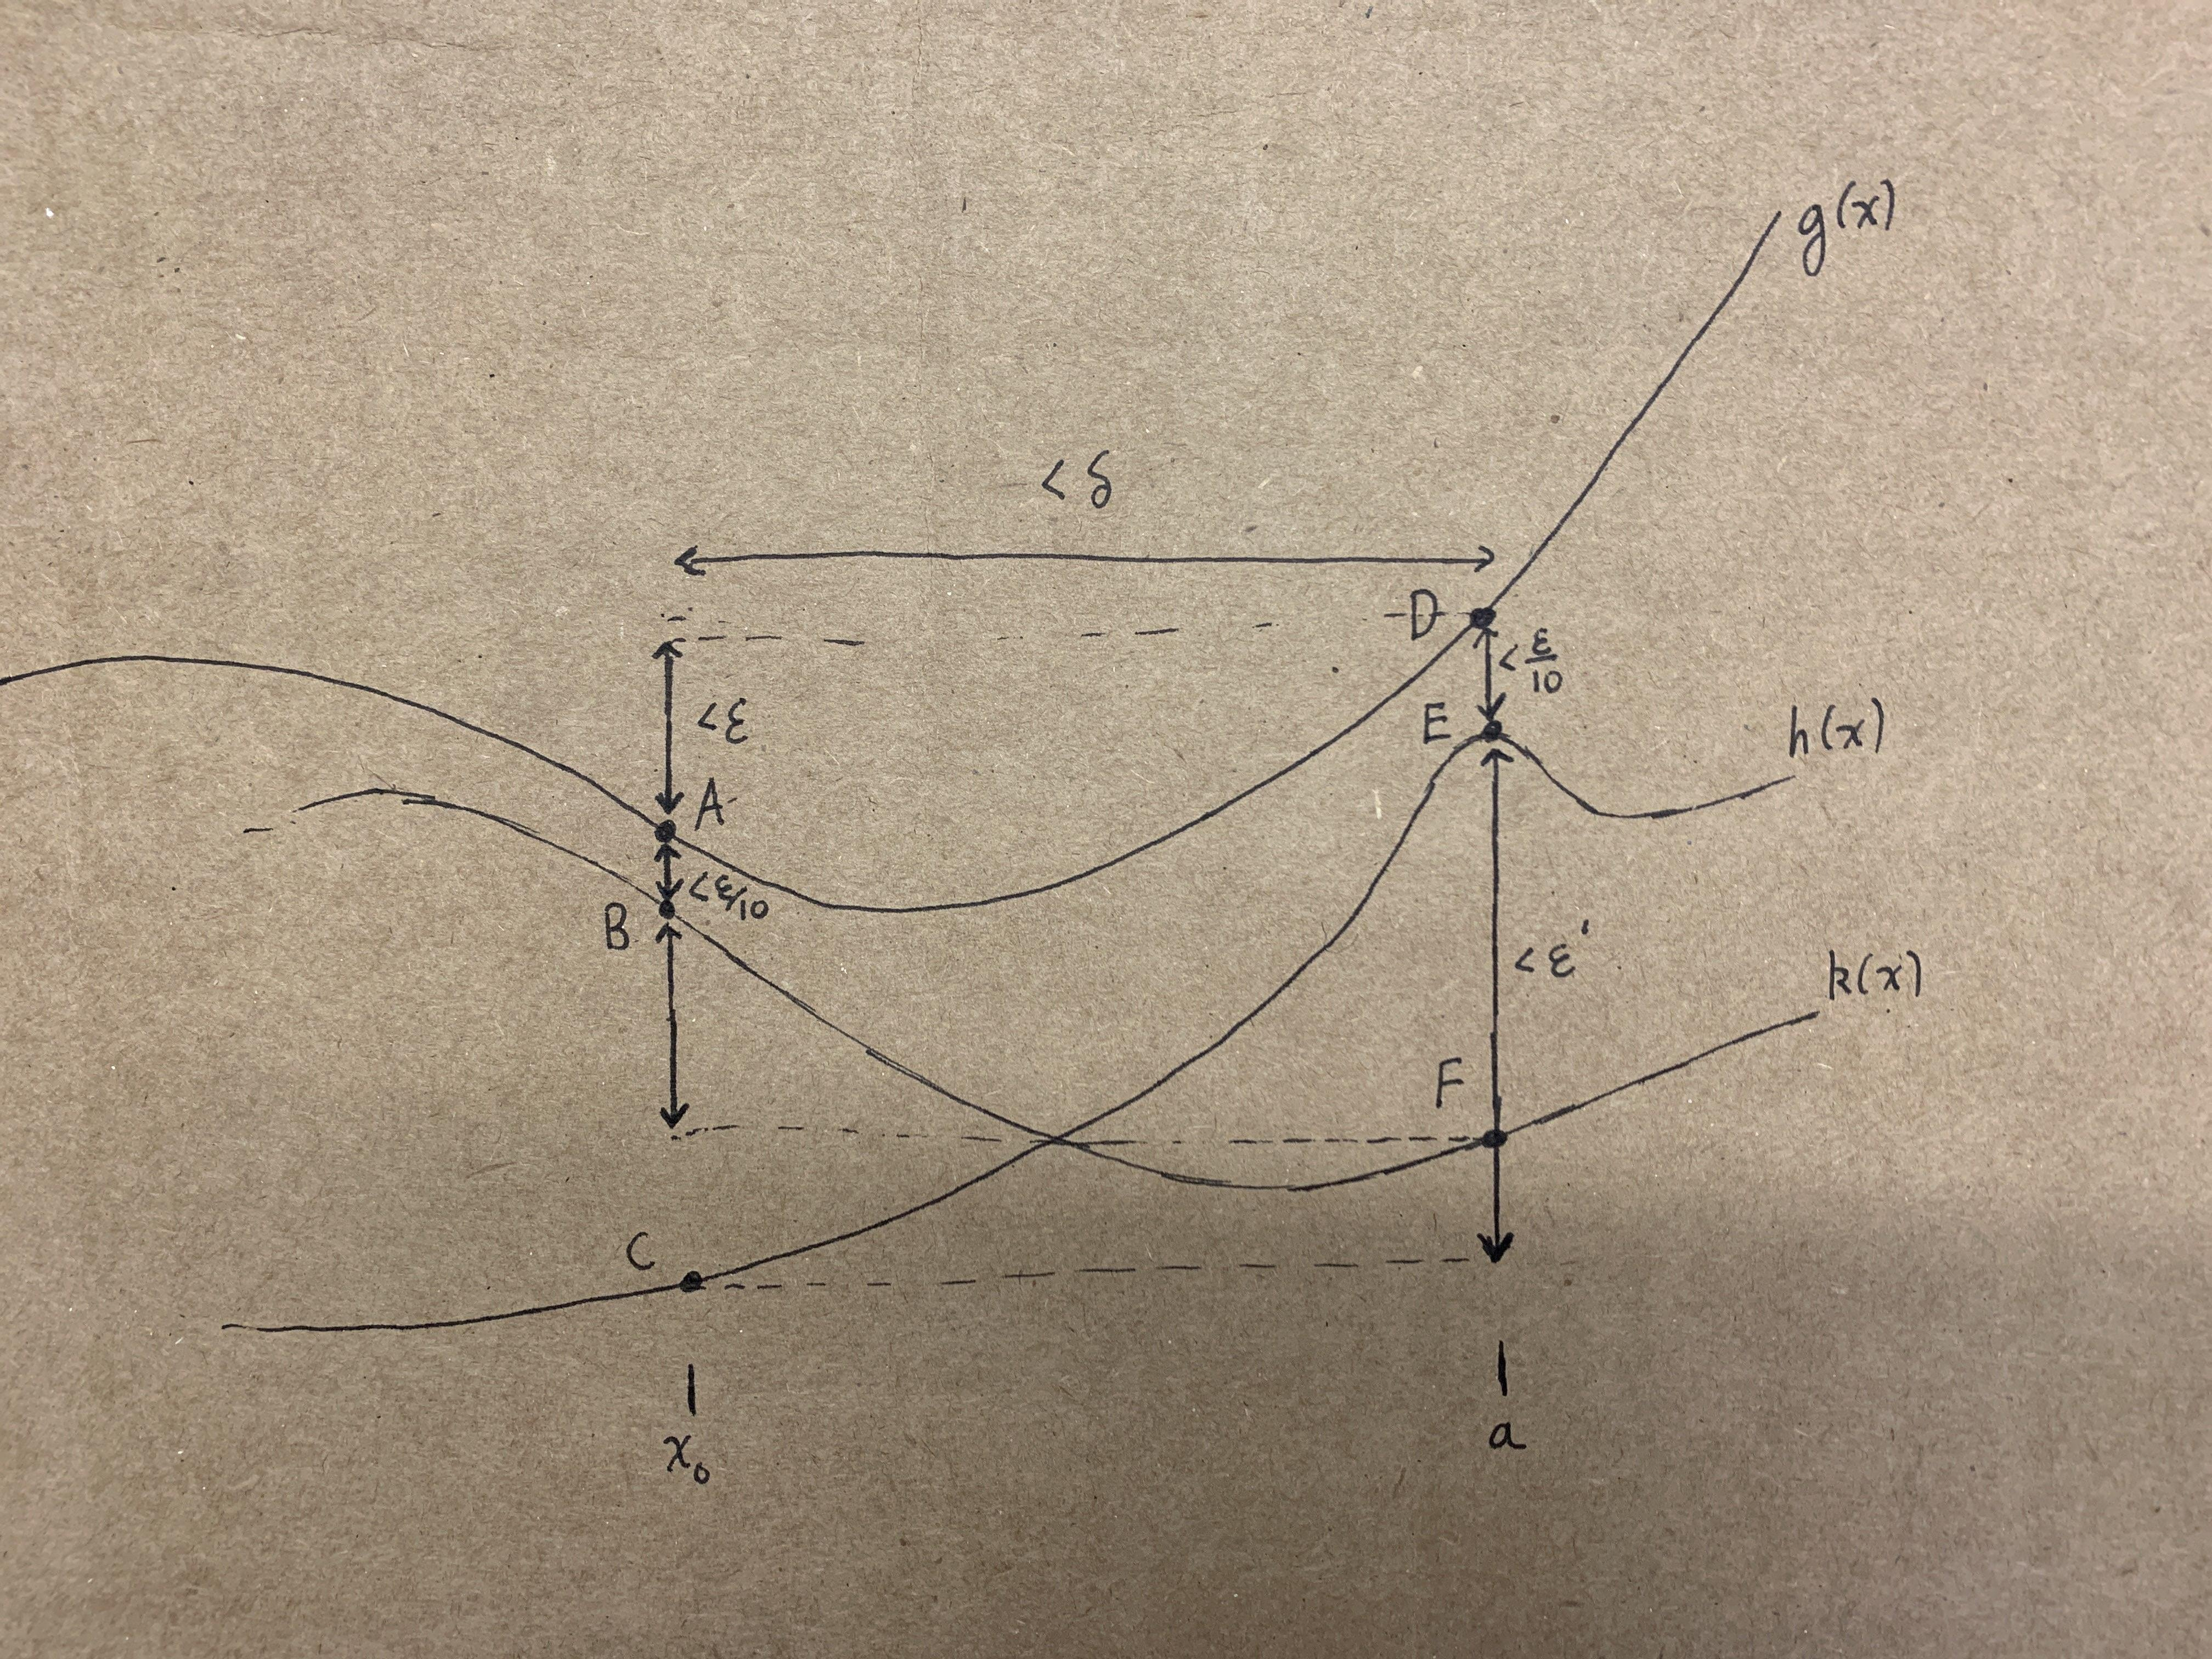
\includegraphics[width=\textwidth]{pset4_4.jpg}
        \end{center}
        Note that if $F$ is above $E$ we will choose $k(x)$ for both graphs and if $C$ is above $B$ then we will chose $h(x)$ for both graphs. Therefore, we can say that $E$ is not below $F$ and $B$ is not below $C.$
    
        We wish to compute $\epsilon:=d(A,D),$ where the norm is the vertical distance. By the triangle inequality, we have:
        \begin{equation}
            d(A,D) < d(A,B)+d(B,F)+d(F,C)+d(C,E)+d(E,D) < \frac{4\epsilon}{10}+d(C,F),
        \end{equation}
        where we set $\epsilon' = \frac{\epsilon}{10}.$ We claim that $d(C,F) < \epsilon'.$ Suppose that $C$ is below $F.$ Then $d(C,F) < d(C,E) < \epsilon/10.$ If instead $C$ was above or at the same height as $F,$ then $d(C,F) < d(F,B) < \epsilon/10.$ Therefore:
        \begin{equation}
            d(A,D) < \frac{5\epsilon}{10} < \epsilon.
        \end{equation}
        Therefore, we showed that $|x_0-a|<\delta$ implies that $d(A,D)=|g(x_0)-g(a)|<\epsilon.$
        \item Consider the sequence
        \begin{equation}
            f_n(x) = \begin{cases}
                -x^n & 0<x \le 1 \\ 
                -(2-x)^n & 1<x<2 \\ 
                0 & \text{else}.
            \end{cases}
        \end{equation}
        It is easy to check that this is continuous for all $n.$ It is bounded, and it is not equicontinuous. To prove failure of equicontinuity of $x^n$ in the closed interval $[0,1]$, pick $\epsilon = 1$ and pick an arbitrary $\delta > 0,$ along with $t,s\in[0,1].$ WLOG, let $t>s$ such that we can write $t=s+\chi,$ where $\chi > 0.$ We can write the inequality:
        \begin{align}
            t^n-s^n &= (s+\chi)^n - s^n \\ 
            &\ge s^n + ns^{n-1}\chi - s^n \\ 
            &= ns^{n-1}\chi .
        \end{align} 
        This shows that for any $s,t$ we pick, we can make the difference $t^n-s^n$ as big as we want since the difference is controlled by $n.$
        
        Now we can compute,
        \begin{equation}
            g(x):=\text{sup}\{f_n(x):n\in \mathbb{N}\} = \begin{cases}
                -1 & x = 1\\ 
                0 & \text{else}.
            \end{cases}
        \end{equation}
        This is true since we will always have $f_n(1)=-1,$ and $f_n(x)=0$ for all $x \le 0$ and $x\ge 2.$ For everything else, $0$ will always be the least upper bound since for any $\epsilon,$ there exists $N\in \mathbb{N}$ such that $f_N(a)>0-\epsilon$ for some $a\in (0,2) \setminus \{1\}.$ Clearly, $g(x)$ is not continuous at $x=1,$ so we have found a counterexample.
        \item See part (d)
        \item Consider the sequence 
        \begin{equation}
            p_n(x) = - f_n(x), 
        \end{equation}
        where $f_n(x)$ is defined as in part (b). This is not equicontinuous for the same reasons. We just need to show that the supremum of the sequence is always continuous. First, note that $p_n(x)$ is a non-increasing monotonic sequence, i.e. 
        \begin{equation}
            p_1(x) \ge p_2(x) \ge \cdots \ge p_n(x)
        \end{equation}
        so if we pick any subset, and we order it by indices, then let $k$ be the smallest index. By monotonic, we have that $p_k(x)$ is the supremum of the subset and since $p_k(x)$ will always be continuous, the spremum-sup property is true for any subset of $\{p_n(x)\}.$
    \end{enumerate}
    \newpage
    \item \begin{enumerate}[label=(\alph*)]
        \item We prove it for a general compact metric space. Consider the sequence $f_n-f.$ Since it is defined on a compact metric space and $f_n-f$ is continuous, it is bounded, and the maximum exists, i.e. 
        \begin{equation}
            \text{sup}\{f_n-f\} = \text{max}\{f_n-f\}.
        \end{equation}
        Also note that $f_n$ is monotonic, so we have $f_n-f$ is monotonic, and it is bounded below by $0.$ Finally, because $f_n$ approaches $f,$ we know that $f_n-f$ approaches $0$ pointwise. If we can show that $f_n-f$ approaches $0$ uniformly, theen we're done. We've now reduced our problem to something simpler:

        Consider monotonically non-increasing sequence $g_n(x),$ where $g_n(x)\ge0$ is bounded, continuous, and defined on a compact set $M$, where $g_n$ approaches $0$ point-wise. We will show that $g_n$ approaches $0$ uniformly. To do so, we will construct an open cover for $M.$ Recall that because $g_n(x)$ approaches point-wise to $0,$ for every $x_\alpha \in M$ there exists an open ball $B_{\delta}(x_\alpha)$ such that for any $\epsilon>0$ there exists $N\in \mathbb{N}$ such that $n>N$ implies that
        \begin{equation}
            \text{sup}\{g_n(x):x\in B_{\delta}(x_\alpha)\} < \epsilon,
        \end{equation}
        which follows immediately from continuity of $g_n(x).$ That is, for any $\epsilon'=\epsilon/2 > 0,$ there exists $\delta > 0$ such that $x\in B_{\delta}(x_\alpha) \implies d(g_n(x),g_n(x_\alpha)) < \frac{\epsilon}{3}.$ But $d(g_n(x),0) < d(g_n(x),g_n(x_\alpha))+d(g_n(x_\alpha),0) < \frac{\epsilon}{3} + \frac{\epsilon}{3} < \epsilon,$ since by point-wise continuity, $g_n(x_\alpha)$ can be arbitrarily close to $0.$

        We do this for every $x_\alpha \in M$ to construct the open cover,
        \begin{equation}
            \bigcup_\alpha B_{\delta_{\alpha}}(x_\alpha) \supseteq M
        \end{equation}
        but since $M$ is compact, we can find a finite subcover,
        \begin{equation}
            \bigcup_{i=1}^n B_{\delta_i}(x_i) \supseteq M.
        \end{equation}
        Then,
        \begin{align}
            \text{sup}\left\{
                g_n(x):x\in M
            \right\} &=\text{sup}\left\{
                \text{sup}\{g_i(x):x\in B_{\delta_i}(x_i)\}:i=1,2,\dots,n
            \right\} \\ 
            &= \text{max}\left\{
                \text{sup}\{g_i(x):x\in B_{\delta_i}(x_i)\}:i=1,2,\dots,n
            \right\}, 
        \end{align}
        where we were able to use the maximum since there are a finite number of elements. But we have shown that each term is bounded by some $\epsilon_i$ for $n>N.$ Therefore, we have 
        \begin{align}
            \text{sup}\left\{
                g_n(x):x\in M
            \right\} &< \text{max}\{\epsilon_1,\dots,\epsilon_n\}.
        \end{align}
        But these $\epsilon_i$ can be anything, so we let their maximum be $\epsilon.$ Therefore, we have shown that for $n>N$ and $\epsilon >0,$ we have 
        \begin{equation}
            \text{sup}\left\{
                g_n(x):x\in M
            \right\} < \epsilon,
        \end{equation}
        so it uniformly converges.
        \item The proof works in exactly the same way. But instead of considering $f_n-f,$ we now consider $f-f_n.$ The same properties still hold (monotonic non-decreasing sequence, bounded below by $0,$ bounded, continuous), so we can still use the same argument.
        \item Consider the counter-example: 
        \begin{equation}
            f_n(x) = \frac{|x|}{n}.
        \end{equation}
        This is a monotonic sequence that converges to $0,$ but it doesn't converge monotonically. For any $\epsilon > 0$ and any $N\in \mathbb{N}$ we can find $x$ and $n>N$ such that $f(x) > \epsilon,$ namely $n=2N$ and $x=4\epsilon N$ which gives 
        \begin{equation}
            f_{2N}(x) = \frac{4\epsilon N}{2N} > \epsilon.
        \end{equation}
        \item We have already proved it for compact metric spaces in part (a). For general $\mathbb{R}^m,$ it doesn't work for the same reason it doesn't work in part (c). In fact, I can define 
        \begin{equation}
            f_n(x_1,\dots,x_n) = \frac{|x_1|}{n}
        \end{equation}
        and the proof why this doesn't converge uniformly to $0$ is exactly the same as before.
    \end{enumerate}
\end{enumerate}

\end{document}